\chapter{A geometrical description of vortex variability}
\begin{quotation}
  Much of the work contained in this chapter is based upon \citet{Seviour2013a},
  published in \emph{Geophysical Research Letters}, although the analysis
  presented here has been significantly extended.
\end{quotation}

\label{cha:moments}

% To Do: 
% - Discussion of sensitivity of the clustering algorithm
% - Description of dripping paint plot
% - Significance for dripping paint plot
% - CP07 and M13 events in table (or maybe disagreeing events highlighed
%   - plot disagreeing events seperately to check
% - Possibly add seasnal cycle of moment diagnostics with percentiles 



\section{Introduction}

A quantitative description of stratospheric polar vortex variability is
desirable for a number of reasons; it allows for the comparison of different
studies, observational data sets, and model simulations, as well as permitting
robust definitions of extreme events.  Traditional methods to quantify vortex
variability have been based on zonal-mean diagnostics, such as the zonal-mean
zonal wind \citep[e.g.,][]{Andrews1987}. This was motivated both by the
simplicity of these diagnostics and the physical reasoning that the strength of
the zonal flow controls the propagation of planetary waves \citep[][Section
\ref{sec:plan-waves-strat}]{Charney1961}. \citet{McInturff1978} provided the
first quantitative definition of SSWs\footnote{In the literature, this is often
  called ``the WMO definition''.} (referred to in that text as ``major
stratospheric warmings'') using zonal mean quantities as below.
\begin{quotation}
A stratospheric warming can be said to be major if at 10~mb or below the
latitudinal mean temperature increases poleward from 60 degrees latitude and an
associated circulation reversal is observed (i.e., mean westerly winds poleward
of 60$^{\circ}$ latitude are succeeded by mean easterlies in the same area).
\end{quotation}
A number of variations of this definition have since appeared in the
literature. Most commonly, the temperature gradient criterion has been neglected
and/or zonal wind reversals at a particular latitude (usually $60^{\circ}$N)
used instead of the stricter criterion of a reversal everywhere poleward of
$60^{\circ}$N \citep[e.g.,][]{Labitzke2000, Christiansen2001,
  Reichler2012}. 

Although the reversal of zonal-mean zonal wind is physically relevant for the
propagation of planetary waves, the choice of $60^{\circ}$N and 10~hPa in the
definition of SSWs is less physically significant. Indeed, different numbers of
SSWs are identified if these locations are varied. \citet{Butler2014a} found
that a greater number of events are identified if the threshold is located
either equatorward or poleward of $60^{\circ}$N. Some studies have aimed to
avoid this sensitivity to spatial location by quantifying vortex variability
through empirical orthogonal function (EOF) analysis, using fields over a larger
area. This includes the Northern Annular Mode (NAM) (calculated either from the
three-dimensional geopotential height field \citep{Baldwin2001a} or zonal-mean
geopotential height \citep{Baldwin2009}), EOFs of zonal wind
\citep{Limpasuvan2004}, and vertical profiles of polar cap-averaged temperature
\citep{Kuroda2004}. SSW events are then defined by a threshold in the principal
component of the relevant EOF.

As it has become increasingly recognised that SSWs generally occur as either
split or displaced vortex events, studies have aimed to objectively distinguish
these two types of event. Commonly this has been achieved through Fourier
decomposition of the zonal wave structure. For instance, \citet{Nakagawa2006}
defined SSWs through a polar temperature criterion and then split these events
into two groups depending on whether the 150~hPa Eliassen-Palm (EP) flux prior
to the events was dominated by zonal wavenumber one or two. \citet{Charlton2007}
(hereafter CP07) introduced a new classification method, which does not rely on
Fourier decomposition; first they identified events using the traditional wind
reversal at $60^{\circ}$N, 10~hPa criterion, then they calculated the circulation
around the two largest contours of relative vorticity on the vortex edge. If
these two contours have a circulation ratio of 2:1 or lower the event is
classified as a split, and all other events are automatically classed as
displacements. 

Both Fourier decomposition of the zonal wave structure and the method of
\citet{Charlton2007} rely on an Eulerian framework, with fields analysed at a
fixed spatial location. \citet{Waugh1997} first applied two-dimensional moment
diagnostics (otherwise known as elliptical diagnostics) to the stratospheric
polar vortex to provide an alternative semi-Lagrangian (or vortex-oriented)
framework. These diagnostics are calculated by fitting an ellipse to a contour
and then determining its properties such as the centre, orientation, aspect
ratio, and area (a further diagnostic, excess kurtosis--a measure of the
`peakedness' of the distribution--was introduced by \citet{Matthewman2009}). This
allows the movement and elongation of the vortex to be
quantified. \citet{Waugh1997} also compared these diagnostics to the traditional
Fourier decomposition. He showed that wave 1 and 2 amplitudes relate most
strongly to the displacement and elongation of the vortex respectively, however,
these relationships were not found to be strong, with correlations of daily
values less than 0.5. These weak relationships were attributed to the fact that
planetary wave propagation can be affected by changes in the meridional PV
gradient, even if the vortex shape and location are fixed. Furthermore, the wave
1 amplitude depends to some extent on the elongation of the vortex as well as
the location of the centre (and similarly for the wave 2 amplitude). He
concluded that it is difficult to extract quantitative information about the
shape and location of the vortex based on wave amplitudes alone, highlighting
the advantages of the moment diagnostics.

\citet{Hannachi2010} then applied a hierarchical clustering algorithm to daily
values of the area, centroid latitude, and aspect ratio diagnostics and found
that the vortex falls preferably into three clusters corresponding to
undisturbed, split, and displaced states. These groupings were used by
\citet{Mitchell2013} (hereafter M13) to identify split and displaced vortex
events; if the vortex remained in the split or displaced cluster for at least
five consecutive days it was classified as the corresponding
event. Significantly, as discussed in Section \ref{sec:observ-evid}, M13
demonstrated that split vortex events penetrated deep into the troposphere and
resulted in significant surface anomalies, while anomalies associated with
displaced vortex events do not descend far below the tropopause. This is in
agreement with \citet{Nakagawa2006} who found tropospheric anomalies to be
larger following SSWs with dominant wave 2 amplitude, however, it contrasts with
\citet{Charlton2007}, who found little difference in the tropospheric impact of
split and displaced vortex events. This highlights the potential importance of
the method of classification of split and displaced vortex events in any study.

In this chapter we wish to develop a method for the classification of split and
displaced vortex events with the following properties:
\begin{enumerate}
\item Based on vortex moment diagnostics.
\item Can be easily applied to a range of data sets, including climate model
  simulations.
\item Computationally inexpensive. 
\end{enumerate}
The motivation for the use of moment diagnostics includes their advantages in
quantifying the shape and location of the vortex, as noted above. This, in turn,
is desireable because the location of the vortex near the tropopause may be
important for understanding the regional tropospheric effect of stratospheric
anomalies \citep[e.g.,][Section \ref{sec:mechanisms}]{Ambaum2002}. Previous
calculations of vortex moment diagnostics have been based on the distributions
of quasi-conservative tracers such as PV on isentropic surfaces
\citep{Mitchell2011} or long-lived tracer (e.g., N$_{2}$O) concentrations
\citep{Waugh1997}. These quantities have strong meridional gradients allowing
for clear determination of the vortex edge \citep{Nash1996}. Unfortunately, many
climate models do not output PV or tracer concentrations, and these are often
computationally expensive or impractical to calculate. As such, we wish to
develop a method which uses geopotential height, a variable which is output by
all contemporary climate models. This effort will also allow us to test the
robustness of the result of M13 regarding the different surface impacts of split
and displaced vortex events using a semi-independent classification method and
extended data set.

The remainder of this chapter is structured as follows. The next section
introduces the necessary theoretical background for the calculation of moment
diagnostics. Section \ref{sec:methodology} describes the methods used for the
classification of split and displaced vortex events, and compares these events
with those determined by M13 and CP07. Section \ref{sec:moments_analysis}
contrasts the surface impacts of split and displaced vortex events calculated
using the new method and discusses potential mechanisms behind any differences. 


% Stratospheric sudden warmings (SSWs) are extreme events in which the strong
% westerly winds that usually dominate the winter polar stratosphere become highly
% disturbed (here, for reasons outlined below, we use the term SSW to encompass a
% wider range of variability than its traditional definition). These events lead
% to the mixing of mid-latitude air into the polar vortex region, causing an
% increase in temperatures by several tens of kelvin over the course of a few
% days. Traditional methods to identify stratospheric sudden warmings (SSWs) have
% relied on either zonal-mean \citep{Andrews1987} or annular mode
% \citep{Baldwin2001a} diagnostics. Neither method explicitly deals with the
% inherent zonal asymmetry in vortex variability. In particular, SSWs are observed
% to occur in one of two manners: displaced vortex events, where the vortex moves
% far from the pole, and split vortex events, where the vortex separates into two
% `child' vortices. These two types have a very different spatial structure and
% evolution timescale \citep{Matthewman2009}. Displaced and split vortex events
% are predominantly associated with vertically propagating Rossby waves of
% wavenumber 1 and 2 respectively, and many previous studies have classified SSWs
% based on wavenumber \citep[e.g.][]{Nakagawa2006}. However, this method does not
% provide a description of the location of the polar vortex itself, which
% theoretical arguments suggest may be important for understanding
% stratosphere-troposphere coupling \citep{Ambaum2002}. In an improvement to these
% traditional SSW definitions, \citet{Charlton2007a} (hereafter CP07) introduced a
% classification in which a split vortex event is identified when two vortices
% with a circulation ratio of 2:1 or higher are present, and all other SSWs are
% automatically classed as displaced vortex events. However, they maintained the
% traditional SSW identification which requires there to be a reversal of the
% zonal-mean zonal wind at 10~hPa and $60^{\circ}$N.

% An increased understanding of stratospheric variability can be gained by using
% vortex-centric diagnostics, such as two-dimensional (2D) vortex moments
% \citep{Waugh1997, Waugh1999, Mitchell2011, Mitchell2011a}, which provide a
% geometrical description of the vortex and have no reliance on zonal-mean
% properties. Using a classification based on these diagnostics,
% \citet{Mitchell2013} (hereafter M13) identified a greater number of SSWs than
% CP07. This is primarily because they did not use a zonal mean threshold
% criterion. Importantly, M13 also demonstrated that split vortex events
% penetrated deep into the troposphere and resulted in significant surface
% anomalies, while anomalies associated with displaced vortex events do not
% descend far below the tropopause. Their result supported a similar conclusion by
% \citet{Nakagawa2006}, who found that the impact of events associated with an
% enhanced upward flux of wavenumber-2 planetary waves was more likely to reach
% the surface. These results underline the need to correctly identify the precise
% type of SSW, in order to understand stratosphere-troposphere coupling within
% climate models.

% Distinguishing between displaced and split vortex events using the method of M13
% requires the use of potential vorticity (PV), which is not commonly output by
% climate models. For this reason, previous attempts to apply PV-based techniques
% in a multi-model study have led to the majority of models being excluded
% \citep{Mitchell2012a}. Furthermore, their method used a hierarchical clustering
% technique \citep{Hannachi2010}, which is very sensitive to the exact shape of
% the distribution of vortex variability, so is unsuitable for application to a
% range of models with different climatologies. In this chapter, we develop an
% improved method which; (a), is based on the geometry of the vortex, but requires
% only the 10~hPa geopotential height; and (b), identifies events using a simple
% threshold instead of a clustering technique. We apply this new method to the
% ERA-40 and ERA-Interim reanalysis datasets and demonstrate that the method
% captures a similar number of events which are in good agreement with, and at
% least as extreme as, those of M13.

\section{Vortex moment diagnostics}
\label{sec:vort-moment-diagn}

The moments, $M_{n}$, of a one-dimensional distribution can be classified by
their order, $n$, and provide familiar parameters. These are the area under the
distribution (0th order), mean (1st order), variance (2nd order), skewness (3rd
order), and kurtosis (4th order), given by
\begin{equation}
M_{n} = \int_{S} x^{n}f(x)\mathrm{d}x \, ,
\end{equation}
where $S$ represents the extent of the distribution, $f(x)$, to be integrated
over. The extension of this for a two-dimensional distribution is
straightforwardly
\begin{equation}
M_{nm} = \iint_{S} x^{n}y^{m}f(x,y)\mathrm{d}x\mathrm{d}y \, ,
\label{eq:2D_moment}
\end{equation}
where the order of the moment is now defined as $m+n$, meaning it is possible to
have different diagnostics with the same order (e.g., $M_{01}$,
$M_{10}$). Although these diagnostics can be further extended to three
dimensions, this has been demonstrated to be highly computationally expensive
\citep{Li1994}, and would require assumptions about the lower and upper bounds
of the vortex region. We therefore calculate two-dimensional moment diagnostics
for the stratospheric polar vortex on quasi-horizontal surfaces. We use two
variables; geopotential height ($f(x,y) = Z(x,y)$) on the 10~hPa pressure level,
and potential vorticity ($f(x,y) = q(x,y)$) on the 850~K potential temperature
(isentropic) surface, which lies close to 10~hPa. Following \citet{Waugh1997},
the calculation of moment diagnostics is simplified by transforming the
spherical data $q(\phi,\lambda)$ and $Z(\phi,\lambda)$, where $\phi$ is latitude
and $\lambda$ longitude, to cartesian coordinates using the polar stereographic
projection
\begin{equation}
x = \frac{\cos\lambda\cos\phi}{1 \pm \sin\phi}\, , \quad
y = \frac{\pm\sin\lambda\cos\phi}{1 \pm \sin\phi}\, , 
\end{equation}  
where the positive sign is used in the Northern Hemisphere and negative in the
Southern Hemisphere.

In order to calculate moment diagnostics for the stratospheric polar vortex we
must first isolate the vortex region by defining the vortex edge. Different
methods have previously been used for this calculation; \citet{Waugh1999} used
the mean PV at the maximum of the mean meridional PV gradient, while
\citet{Matthewman2009} defined the vortex edge on a daily basis, using the
average value of PV poleward of $45^{\circ}$N nine days before the onset of a
SSW (their SSWs were defined by zonal-mean zonal wind reversal, as in CP07). A
more complex method due to \citet{Nash1996}, starts by transforming PV to
`equivalent latitude' \citep{Butchart1986} coordinates, before defining the
vortex edge as the position of the largest gradient in a plot of PV against
equivalent latitude. This method was applied in \citet{Mitchell2011} to
calculate the vortex edge. 

None of the three methods outlined above are found to be appropriate for the
present study. We wish to directly compare the PV and geopotential
height-derived moments, but the methods of \citet{Waugh1999} and
\citet{Nash1996} rely on meridional gradients in PV and so may not be
transferable to geopotential height. Furthermore, the method of
\citet{Matthewman2009} is impractical because we wish to define the events from
the moment diagnostics, so will not know their dates before
calculation. Instead, we pick a simple definition; PV ($q_{b}$) or geopotential
height ($Z_{b}$) on the vortex edge is defined as the value of the
December-March (DJFM) mean at $60^{\circ}$N for the Northern Hemisphere and the
June-September (JJAS) mean at $60^{\circ}$S for the Southern Hemisphere. This is
seen to lie close to contours defined by the above methods, and results are
insensitive to small changes in the latitude chosen.

Having defined the vortex edge, we extend the method \citet{Matthewman2009} to
isolate the vortex region by introducing a transformed PV field, $\hat{q}$,
given by
\begin{equation}
 \hat{q}(x,y) = 
 \begin{cases}
   q(x,y) - q_{b} & \text{if $q(x,y) > q_{b}$} \, , \\
   0 & \text{if $q(x,y) \leq q_{b}$} \, , 
 \end{cases}
\end{equation}
and similarly for geopotential height 
\begin{equation}
 \hat{Z}(x,y) = 
 \begin{cases}
   Z(x,y) - Z_{b} & \text{if $Z(x,y) < Z_{b}$} \, , \\
   0 & \text{if $Z(x,y) \geq Z_{b}$} \, . 
 \end{cases}
\end{equation}
By substituting $f(x,y) = \hat{q}(x,y)$ or $f(x,y) = \hat{Z}(x,y)$ in equation
\ref{eq:2D_moment} it is then possible to calculate the moment diagnostics. The
zeroth order moment diagnostic, $M_{00}$ can be used to define the `equivalent
area', $A_{\mathrm{eq}}$ \citep{Matthewman2009}, as
\begin{equation} 
A_{\mathrm{eq}} = \frac{M_{00}}{q_{b}}\quad \text{or} \quad A_{\mathrm{eq}} = \frac{M_{00}}{Z_b}\, ,
\end{equation}
depending on whether PV or geopotential height based diagnostics are
calculated. Because $M_{00} \approx Aq$, where A is the vortex area, the
equivalent area can be considered a measure of both vortex strength and
area. The first order moment diagnostic can be used to calculate the vortex
centroid,
\begin{equation}
(\bar{x}, \bar{y}) = \left( \frac{M_{10}}{M_{00}}, \frac{M_{01}}{M_{00}} \right)
\, . 
\end{equation}

In order for higher order moment diagnostics to be useful, the moment equation
(\ref{eq:2D_moment}), must be transformed to the \emph{centralised moment}
form \citep{Hall2005}. This calculates moments relative to the vortex centroid,
and is given by
\begin{equation}
J_{mn} = \iint_{S} f(x,y)(x-\bar{x})^n(y-\bar{y})^m\mathrm{d}x\mathrm{d}y \, .
\end{equation}
Two useful parameters can be derived from the second-order centralised moment
diagnostics, the vortex orientation, $\psi$ (defined as the angle between the
major axis of the ellipse and the $x$-axis) and the aspect ratio, $r$ (defined
as the ratio of the lengths of the major to minor axes), given by
\begin{equation}
\psi = \frac{1}{2} \tan^{-1} \left( \frac{2J_{11}}{J_{20}-J_{02}} \right) \, ,
\end{equation}
\begin{equation}
r = \left| \frac{(J_{20}+J_{02})+\sqrt{4J_{11}^2+(J_{20}-J_{02})^2}}
  {(J_{20}+J_{02})-\sqrt{4J_{11}^2+(J_{20}-J_{02})^2}} \right|^{1/2} \, .
\end{equation}
Using the area, centroid, orientation, and aspect ratio, the \emph{equivalent
  ellipse} can be uniquely defined. Figure \ref{fig:displaced_ellipse} shows the
equivalent ellipse calculated from both PV and geopotential height fields over a
16-day period centred on a displaced vortex event (classified using the method
in Section \ref{sec:methodology}). It can be seen that the equivalent ellipse
provides a qualitatively good fit to the vortex, although this is less good in
Figures \ref{fig:displaced_ellipse}(c,f) when the vortex becomes less elliptical
and filamentation occurs. Greater fine-scale structure and filamentation is
visible in the PV field due to its quasi-conservative properties, however
reasonable agreement can be seen between the PV and geopotential height
ellipses. 

\begin{figure}
 \centering
 \noindent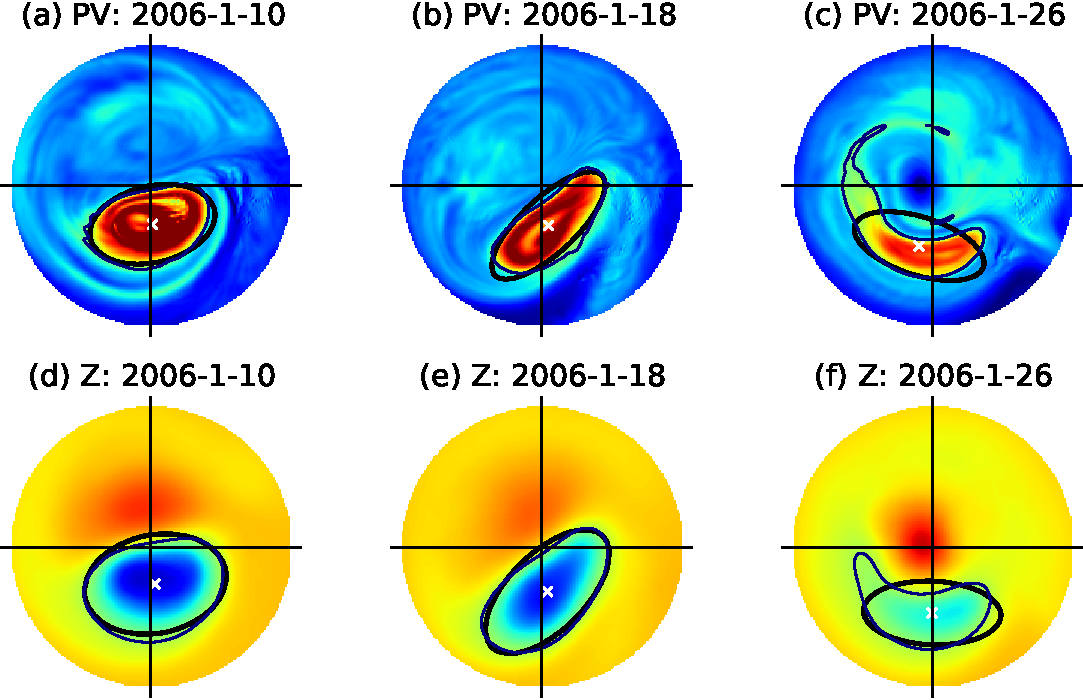
\includegraphics[width=\textwidth]{figures/chapter-moments/PV_GPH_2006.pdf}
 \caption[Equivalent ellipse for a displaced vortex event.]{PV on the 850~K
   $\theta$ surface (a,b,c) and geopotential height at 10~hPa (d,e,f) 8 days
   before (a,d), at onset (b,e), and 8 days following the onset (c,f) of a
   displaced vortex event. Contours of $q_{b}$ and $Z_{b}$ are shown in thin
   black lines, the equivalent ellipse in a thick dark line, and its centroid
   with a white cross. Data are transformed to cartesian coordinates with a
   polar stereographic projection.}
 \label{fig:displaced_ellipse}
\end{figure}

Equivalent ellipses for an example of a split vortex event are shown in Figure
\ref{fig:split_ellipse}. It can be seen that after the vortex has separated the
equivalent ellipse becomes less physically significant, as it spans the two
vortices. \citet{Matthewman2009} introduced the 4th order moment diagnostic,
``excess kurtosis'', in order to identify splits of the polar vortex; it is
given by
\begin{equation}
\kappa_4 = M_{00}\frac{J_{40}+2J_{22}+J_{04}}{(J_{20}+J_{02})^2}-\frac{2}{3}\left[\frac{3r^4+2r^2+3}{(r^2+1)^2}\right]\,.
\end{equation}
This has the property of being negative for a vortex with a ``pinched'' shape,
zero for a perfectly elliptical vortex, and positive for a vortex with a strong
central core. When negative kurtosis was detected \citet{Matthewman2009} split
the PV field into two regions along the minor axis of the equivalent ellipse and
re-calculated moment diagnostics for the vortices in these regions separately. 

In this study we do not make use of the excess kurtosis or calculate separate
diagnostics for split vortices for two reasons. First, as a 4th order diagnostic
it is a highly skewed variable, making its use in event classification
problematic (this was also found by \citet{Hannachi2010}). Second, this
procedure is more computationally expensive, requiring about three times the
number of calculations during split vortex events. Hence, we calculate single
moment diagnostics even when the vortex has split, but bear in mind that these
may not represent the properties of any real vortex. 

Code for the calculation of moment diagnostics using the method described
in this section is available from
\url{https://github.com/wseviour/vortex-moments}.

\begin{figure}
 \centering
 \noindent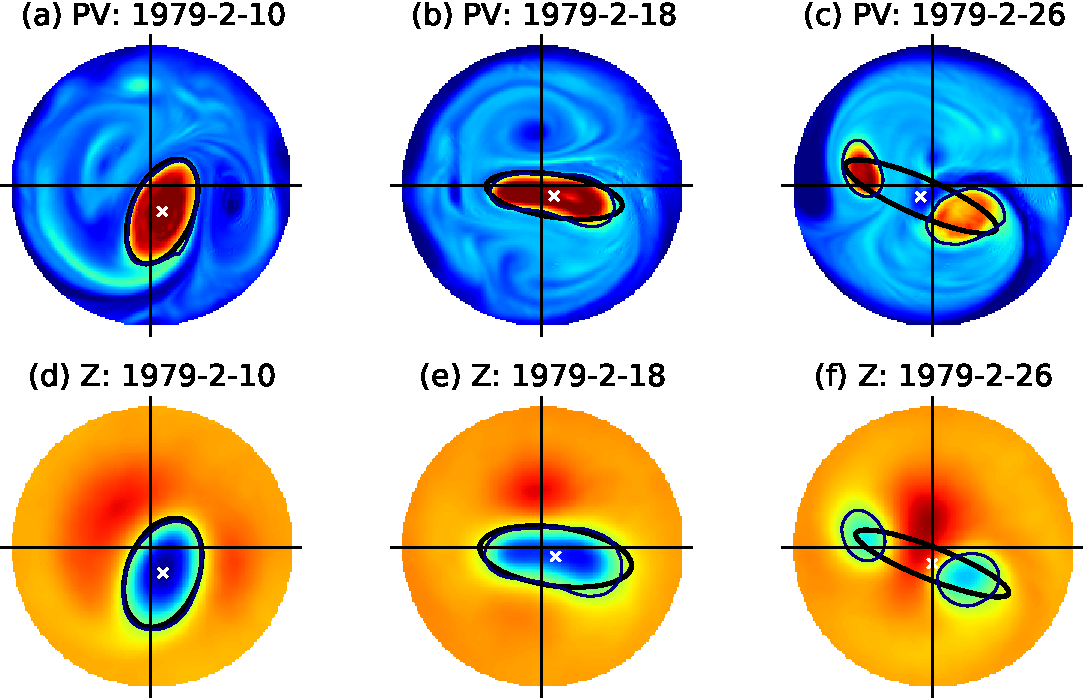
\includegraphics[width=\textwidth]{figures/chapter-moments/PV_GPH_1979.pdf}
 \caption[Equivalent ellipse for a spit vortex event.]{As Figure
   \ref{fig:displaced_ellipse} but for a split vortex event.}
 \label{fig:split_ellipse}
\end{figure}


\section{Data and methods}
\label{sec:methodology}

\subsection{Reanalysis data}

For the analysis in this chapter Northern Hemisphere winter daily-mean data for
December-March (DJFM) are employed from the European Centre for Medium-Range
Weather Forecasts (ECMWF) reanalyses. The ERA-40 data set \citep{Uppala2005} is
used from 1958-1978 and ERA-Interim \citep{Dee2011} from 1979-2009. The
combination of these two data sets is chosen in order to maximise the total
number of years entering the analysis (ERA-40 runs only to 2002), as well as to
compare results from the more recent ERA-Interim with previous studies using
only ERA-40, such as \citet{Charlton2007} and \citet{Mitchell2013}.

ERA-Interim is similar to ERA-40 but uses ECMWF’s operational four-dimensional
variational data assimilation system (4D-Var) as opposed to the 3D-Var system
used in ERA-40. It also has higher horizontal and vertical resolution, improved
humidity analysis, model physics, data quality control, bias handling and other
improvements as noted in \citet{Simmons2007}. The majority of observational data
for the stratosphere entering both reanalyses is from radiosonde and satellite
measurements. It is important to note that in the pre-satellite era (1958-1971)
observations in the stratosphere were much more sparse, leading to greater
errors in reanayses during this time \citep{Uppala2005}. 

A number of studies have evaluated the stratospheric circulation in ERA-40 and
ERA-Interim against other observations or reanalyses. \citet{Randel2004} found
ERA-40 to closely match measurements of the zonal stratospheric circulation
derived from radiosonde, rocketsonde and lidar
measurements. \citet{Karpetchko2005} found that the representation of the polar
vortices in ERA-40 agrees well with the NCEP/NCAR reanalysis, and CP07
demonstrated that this also holds for the occurrence of
SSWs. \citet{Seviour2012} showed that the strength of the stratospheric
meridional mean stratospheric circulation in ERA-Interim agrees well with
previous reanalysis, but that the residual vertical velocity is more smoothly
represented.

In order to perform a consistent analysis across the two data sets, ERA-Interim
data is linearly interpolated to the lower resolution ERA-40
($1.125^{\circ} \times 1.125^{\circ}$) Gaussian grid. PV is also interpolated
from pressure levels to the 850~K isentropic surface (which lies close to
10~hPa), as this quantity has the property of being conserved under adiabatic
flow. In the calculation of the vortex edge. Both in the calculation of the
vortex edge (climatological mean $q$ or $Z$ at $60^{\circ}$N/S) and the moment
diagnostics themselves, no clear jumps were seen between ERA-40 and ERA-Interim
data sets. As such, the two are considered together with no bias
corrections. For the remainder of this thesis, this combined ERA-40 and
ERA-Interim data set is referred to as `ERA'. 


\subsection{Moment diagnostic calculation}
\label{sec:vort-geom-calc}

In order to calculate the moment diagnostics, the values of PV and geopotential
height on the vortex edge ($q_b$ and $Z_b$) must first be determined. These are
the $60^{\circ}$N DJFM/$60^{\circ}$S JJAS mean values of PV at 850~K ($q_{850}$)
and 10~hPa geopotential height ($Z_{10}$) respectively. They are found to be
$q_b = 460$~PVU ($\mathrm{1~PVU = 10^{-6}Km^2kg^{-1}s^{-1}}$) and
$Z_b = 30.2$~km for the Northern Hemisphere, and $q_b = 618$~PVU and
$Z_b = 29.0$~km for the Southern Hemisphere. Using these values the moment
diagnostics are calculated from ERA data for 1958--2009 using the method
described in Section \ref{sec:vort-moment-diagn}.

As discussed in Section \ref{sec:vort-moment-diagn} the excess kurtosis
diagnostic is not used in the present analysis. In the interests of simplicity,
only the aspect ratio and centroid latitude diagnostics are used to identify
events, and the centroid longitude, orientation and equivalent area are not
used. The aspect ratio and centroid latitude are the most intuitive diagnostics
for this purpose, with a high aspect ratio and poleward centroid latitude
expected during split vortex events, and a low aspect ratio and equatorward
centroid latitude expected during displaced vortex events. 

Figure \ref{fig:pv_z_moments_distribution} shows the distributions of these two
quantities calculated from $q_{850}$ and $Z_{10}$ for the Northern Hemisphere
vortex. The centroid latitude distributions are almost identical, with a peak
near $80^{\circ}$N which is in agreement with previous studies
\citep{Mitchell2011,Waugh1999}. The aspect ratio distributions have a similar
shape, with a peak at about 1.3, but the PV based diagnostic has a larger
tail. This is because the PV field contains more small-scale filamentary
structures than geopotential height (e.g. Figures \ref{fig:displaced_ellipse}
and \ref{fig:split_ellipse}), making high aspect ratios more likely. As well as
having similar distributions, the time series of the PV and geopotential height
derived diagnostics (not shown) are significantly correlated, with correlation
coefficients of 0.9 for daily centroid latitude and 0.6 for aspect
ratio. Overall, these results suggest that geopotential height-derived moment
diagnostics are appropriate for the identification of split and displaced vortex
events.


\begin{figure}
  \centering
  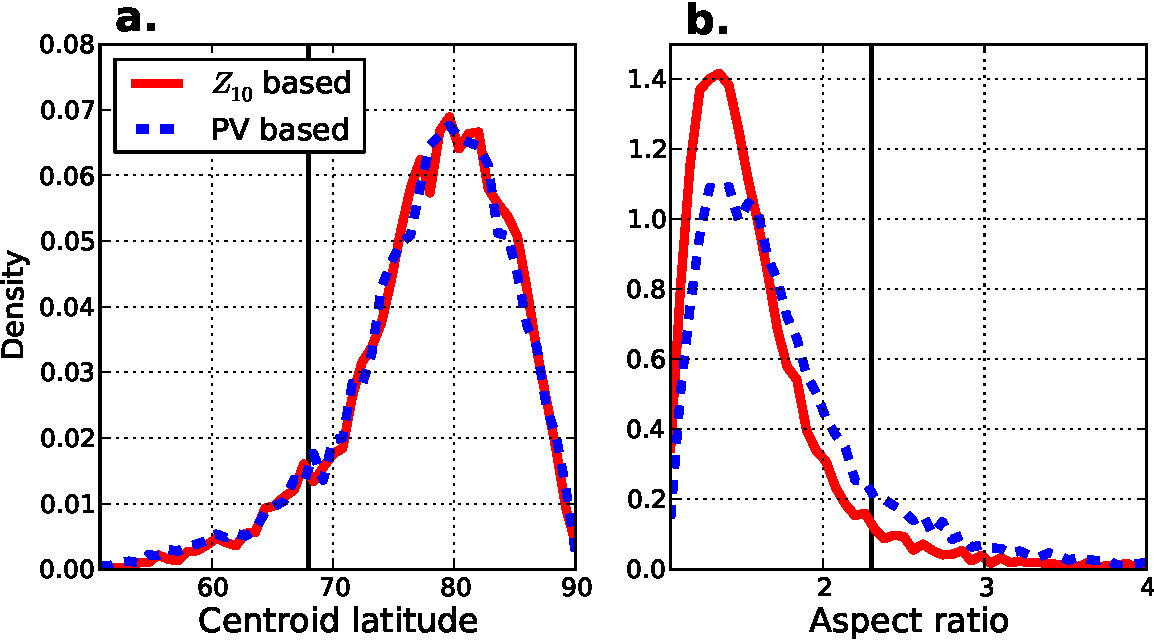
\includegraphics[width=\textwidth]{figures/chapter-moments/moments_distribution_crop.pdf}
  \caption[NH distributions of $Z_{10}$ and PV-based moment
  diagnostics.]{Distributions of the December-March centroid latitude (a) and
    aspect ratio (b), of the Northern Hemisphere stratospheric polar vortex over
    1958-2009. Diagnostics are calculated from geopotential height at 10~hPa
    ($Z_{10}$) and potential vorticity at 850~K (PV). Thresholds of
    66$^{\circ}$N in centroid latitude and 2.4 in aspect ratio are used to
    define events, and are indicated by the black vertical lines.}
  \label{fig:pv_z_moments_distribution}
\end{figure}

\begin{figure}
  \centering
  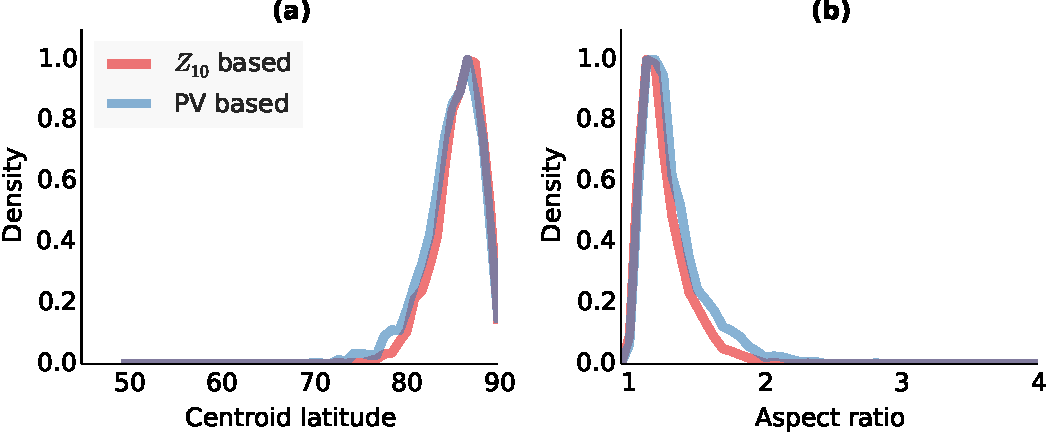
\includegraphics[width=\textwidth]{figures/chapter-moments/moments_distribution_crop_sh.pdf}
  \caption[SH distributions of $Z_{10}$ and PV-based moment diagnostics.]{As
    Figure \ref{fig:pv_z_moments_distribution} but for moment diagnostics
    calculated for the Southern Hemisphere stratospheric polar vortex over
    June-September.}
  \label{fig:pv_z_moments_distribution_sh}
\end{figure}

Figure \ref{fig:pv_z_moments_distribution_sh} shows the same distribution as
Figure \ref{fig:pv_z_moments_distribution}, but for the Southern Hemisphere
vortex aspect ratio and centroid latitude. As in the case of the Northern
Hemisphere, the geopotential height and PV-based distributions have very similar
shapes, with the PV-based aspect ratio having a slightly larger tail. Comparing
the Northern and Southern Hemisphere distributions it can be seen that there is
much less variability in both aspect ratio and centroid latitude in the Southern
Hemisphere. This is because of the reduced planetary wave propagation into the
Southern Hemisphere stratosphere, in turn a result of lesser forcing from
orography and land-sea temperature contrasts. The peak in the Southern
Hemisphere centroid latitude is at about $86^{\circ}$S; the same as that found
by \citet{Waugh1999}. 

A result of this reduced Southern Hemisphere vortex variability is that only one
SSW has been observed in the Southern Hemisphere (discussed further in Chapter
\ref{cha:seas}). The rest of this chapter relates to the classification and
impacts of split and displaced vortex events and so focusses only on the
Northern Hemisphere. However, it should be noted that all the methods below can
also be applied to the Southern Hemisphere.


\subsection{Event identification}
\label{sec:event-definition}

Previous attempts to identify SSW events have used a clustering method
\citep{K.Coughlin2009,Hannachi2010}. These methods attempt to classify the
vortex state for each day into a number of groups, which may be specified
beforehand or determined by the clustering algorithm. Individual days within the
same cluster should be physically similar, while those in different clusters
distinct. More precisely, clustering aims to maximise the between-cluster
variance while minimising the within-cluster variance. In the case of the
stratospheric polar vortex, clusters may represent, for instance, stable, split,
and displaced states. Events are then typically defined by the vortex persisting
in a particular cluster for a number of days.

\begin{figure}
 \centering
 \noindent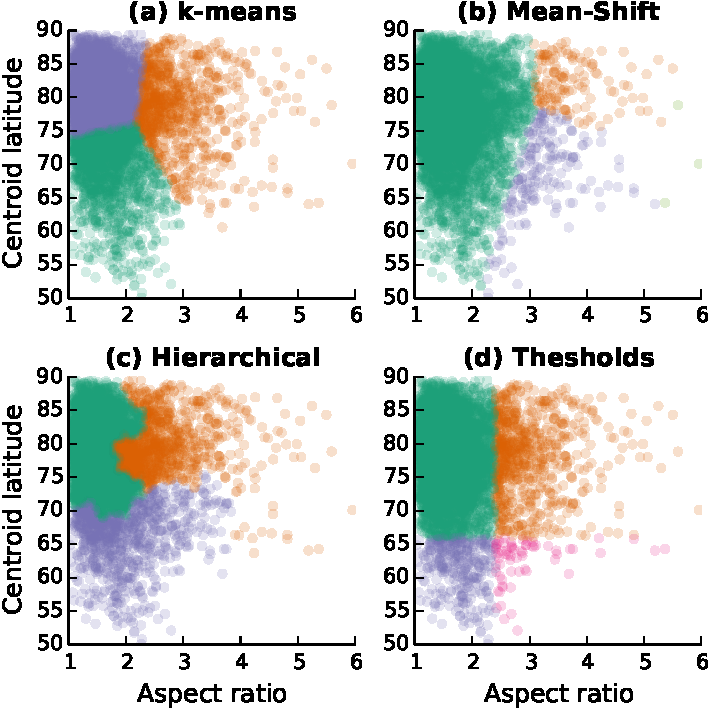
\includegraphics[width=0.7\textwidth]{figures/chapter-moments/clustering.pdf}
 \caption[Clustering algorithms applied to the moment diagnostics.]{Three
   clustering algorithms and a threshold division applied to the moment
   diagnostics in centroid latitude-aspect ratio space. For the $k$-means and
   hierarchical algorithms three clusters were specified. The mean-shift
   algorithm determined the number of clusters to be 4.}
 \label{fig:clusters}
\end{figure}

A large number of clustering algorithms exist, and some may be more appropriate
than others for certain uses. Here, three different algorithms are applied to
the moment diagnostics in centroid latitude-aspect ratio space, and their
outcomes shown in Figure \ref{fig:clusters}(a,b,c). Details of the three
algorithms are given below:
\begin{enumerate}[(a)]
\item \textbf{\textit{K}-means} clustering requires the number of clusters, $K$,
  to be specified beforehand (in Figure \ref{fig:clusters}, $K=3$). The
  algorithm begins by randomly selecting $K$ data points to be the centroids of
  the initial clusters, all other data points are assigned to the cluster with
  the nearest centroid. Having assigned the initial cluster membership, the
  algorithm proceeds as follows:
  \begin{enumerate}[1.]
    \item Compute the centroids (the vector means), $\mathbf{\overline{x}}_k$
      of each cluster. 
    \item Calculate the distance between the current data point, $\mathbf{x}_i$,
      and each of the $K$ $\mathbf{\overline{x}}_k$s. (Various distance measures
      can be used; in Figure \ref{fig:clusters}(a), the Euclidean distance is
      used).
    \item If $\mathbf{x}_i$ is not in the group with the closest mean then
      reassign it to that group, otherwise repeat step 2 for $\mathbf{x}_{i+1}$.
  \end{enumerate}
  This is repeated until a full cycle through each $\mathbf{x}_i$ produces no
  reassignments. An advantage of this method is that it is computationally
  efficient, but the major disadvantage is that the number of clusters must be
  pre-determined. Several methods exist to estimate the ideal number of
  clusters, which generally have the aim of finding the best compromise between
  minimising within-cluster variance and maximising between-cluster
  variance. \citet{K.Coughlin2009} applied $K$-means clustering to several
  variables representing the stratospheric polar vortex. They used a method
  known as silhouette values \citep{Rousseeuw1987} and determined the ideal
  number of clusters to be two (representing stable and disturbed vortex
  states).


\item \textbf{Mean-shift} clustering aims to discover `blobs' in a data set. It
  works by updating candidates for centroids to be the mean of the points within
  a given region. That is, given a candidate centroid $\mathbf{x}_i$ for
  iteration $t$, the candidate is updated according to
  \begin{equation}
    \mathbf{x}^{t+1}_{i} = \mathbf{x}^t_i + \mathbf{m}(\mathbf{x}^t_i) \, ,
  \end{equation}
 where $\mathbf{m}$ is the mean shift vector. This is calculated as
 \begin{equation}
  \mathbf{m}(\mathbf{x}_i) = \frac{\sum_{\mathbf{x}_j \in N(\mathbf{x}_i)}K(\mathbf{x}_j-\mathbf{x}_i)\mathbf{x}_j}{\sum_{\mathbf{x}_j
      \in N(\mathbf{x}_i)}K(\mathbf{x}_j-\mathbf{x}_i)} \, ,
 \end{equation}
 where $K(\mathbf{x}_j-\mathbf{x}_i)$ is a kernel function which determines the
 weight of nearby points. Typically, and in Figure \ref{fig:clusters}(b), a
 Gaussian kernel is used,
 $K(\mathbf{x}_j-\mathbf{x}_i) = e^{-c\|\mathbf{x}_j-\mathbf{x}_i\|^2}$.
 $N(\mathbf{x}_i)$ represents the set of points for which
 $K(\mathbf{x}_i) \ne 0$. This shifting is repeated until $\mathbf{m}$
 converges. Following this calculation, the candidates are then filtered to
 remove near duplicates. The greatest advantage of this method is that it
 automatically sets the number of clusters, so no prior assumptions about the
 data set are required. A disadvantage is that it requires multiple nearest
 neighbour searches during each iteration, and so may not be scalable to large
 data sets. In Figure \ref{fig:clusters}(b) the number of clusters was
 determined to be four. 

\item \textbf{Hierarchical} clustering proceeds by calculating a series of
  nested clusters. To begin with, all data points are considered each as a
  separate cluster and then at each iteration the nearest two clusters are
  merged. There are a number of methods to identify the distance between
  clusters when those clusters consist of more than one member. Following
  \citet{Hannachi2010} the \emph{complete-linkage} method; defining the distance
  as the largest distance between members in the two groups. As with the
  $K$-means clustering, the number of clusters desired must be pre-determined,
  otherwise the algorithm will run to completion with a single cluster
  consisting of all data points. Again, many methods exist to determine the
  optimum number of clusters. \citet{Hannachi2010} used the gap statistic method
  \citep{Tibshirani2001} with vortex area, centroid latitude, and aspect ratio
  moment diagnostics, and found a slight preference for three clusters. As such,
  three clusters are used in Figure \ref{fig:clusters}(c).

\end{enumerate}

Figure \ref{fig:clusters} demonstrates that the three clustering methods produce
very different results. As well as the size and extent of the clusters, there is
also disagreement between this and past studies on the optimum number of
clusters; \citet{K.Coughlin2009} found two clusters using a silhouette values
method, \citet{Hannachi2010} found three clusters using the gap statistic, while
the mean-shift algorithm applied here produces four clusters. Further
sensitivity tests were performed by randomly removing 1\% of the data and
re-calculating the clustering. It was found that very different clusters were
calculated with this small alteration to the data, suggesting that these
clusterings may not be robust if applied to different data sets, such as climate
model simulations. The likely reason for this sensitivity is that the data
itself is not highly clustered; as can be seen in Figure
\ref{fig:pv_z_moments_distribution} no clear bi-modality is present. Rather, it
is more appropriate to view the split and displaced vortex states as the tails
of a distribution rather than distinct clusters or regimes. 

For the reasons above, clustering methods are deemed inappropriate for the
present study, and a simpler, more robust, thresholds-based method is
introduced. Days with an aspect ratio $>2.4$ (11\% of all days) or a centroid
latitude $<66^{\circ}$N (5\% of all days) are classified as split and displaced
states respectively. A small number of days lie beyond both thresholds, and
these are classified as a mixed state (1\% of all days). The vast majority of
days (83\%) lie in the stable state, where neither threshold is exceeded. The
choice of thresholds is somewhat subjective but the results presented below are
not sensitive to the exact choice of threshold. They were chosen to give a
similar frequency of split and displaced vortex events (identified using the
method below) as CP07 and M13. 

\citet{Mitchell2011} found that the aspect ratio and centroid latitude follow an
extreme value distribution \citep{Cole} and it is noted that both thresholds
chosen here lie beyond the extreme value thresholds of their respective
distributions (these were found to be 2.3 for aspect ratio and $72^{\circ}$N for
centroid latitude). Some theoretical motivation for the aspect ratio threshold
can also be provided by the theoretical stability of an idealised elliptical
vortex. \citet{Love1893} found that the Kirchoff ellipse (an elliptical patch of
uniform vorticity in a quiescent fluid) is linearly unstable if the aspect ratio
exceeds 3. The aspect ratio threshold of 2.4 used here lies below this limit,
and so under this idealised model it might expect that some split vortex events
do not display a full separation into two vortices.

\begin{table}
  \begin{centering}
    \begin{tabular}{|l|l|l|l|l|}  \hline
    No. & Event onset & Event type & $\Delta \mathrm{T}_{10}$ (K) &
                                                                    $\overline{U}_{10} (\mathrm{m~s^{-1}})$ \\ \hline
    1*  & 1961-3-9    & D          & 10.2       & 2.7 \\
    2*  & 1962-1-30   & S          & 1.9        & 38.9 \\
    3*  & 1962-3-7    & S          & -1.0       & 16.9 \\
    4*  & 1964-3-15   & D          & 11.9       & 1.3 \\
    5\dagger  & 1966-2-26   & D          & 2.5        & -5.9 \\
    6   & 1967-12-29  & S          & 13.0       & 19.4 \\
    7\dagger   & 1970-1-5    & S          & 8.5        & -4.0 \\
    8   & 1971-1-15   & S          & 10.8       & -1.7 \\
    9*  & 1972-2-4    & S          & -1.6       & 33.6 \\
    10\dagger  & 1973-2-4    & S          & 7.3        & -6.6 \\
    11* & 1974-3-12   & D          & 5.3        & -4.8 \\
    12* & 1975-3-16   & D          & 7.6        & -8.0 \\
    13* & 1976-3-31   & D          & 8.2        & -13.3 \\
    14\dagger  & 1977-1-7    & S          & 7.6        & -5.5 \\
    15*\dagger & 1978-3-25   & D          & 2.5        & -9.3 \\
    16  & 1979-2-18   & S          & 5.6        & -0.4 \\
    17  & 1984-2-25   & D          & 11.6       & -4.4 \\
    18  & 1984-12-25  & S          & 15.0       & -1.7 \\
    19* & 1986-1-7    & S          & 3.4        & 29.9 \\
    20* & 1986-3-21   & D          & 9.1        & -12.2 \\
    21  & 1987-1-20   & D          & 8.3        & -7.7 \\
    22  & 1987-12-10  & S          & 9.8        & -3.0 \\
    23* & 1992-3-22   & D          & 7.6        & -4.4 \\
    24*\dagger & 1995-2-2    & D          & 5.6        & 7.7 \\
    25  & 1998-12-15  & D          & 8.2        & 8.1 \\
    26  & 1999-2-24   & S          & 6.6        & -12.7 \\
    27  & 2001-2-7    & S          & 5.2        & -7.2 \\
    28* & 2001-3-15   & S          & -6.8       & 12.1 \\
    29* & 2002-3-21   & S          & -1.5       & 5.1 \\
    30  & 2003-1-17   & S          & 6.1        & 16.8 \\
    31  & 2004-1-2    & D          & 5.8        & -4.8 \\
    32* & 2005-3-11   & D          & 3.1        & -5.0 \\
    33  & 2006-1-17   & D          & 4.2        & -14.3 \\
    34  & 2008-2-18   & D          & 4.6        & 2.3 \\
    35  & 2009-1-18   & S          & 13.2       & 16.9 \\ \hline
    \end{tabular}
    \caption{A summary table of displaced (D) and split (S) vortex events,
      identified from 10~hPa geopotential height data from 1958-2009.
      $\Delta \mathrm{T}_{10}$ represents the mean area-weighted
      $50^{\circ}$-$90^{\circ}$N cap temperature anomaly at 10 hPa calculated 5
      days either side of the event onset date. $\overline{U}_{10}$ represents
      $\overline{U}$ at $60^{\circ}$N and 10~hPa averaged over the same
      period. Asterisks (*) represent those numbers that do not coincide
      (i.e. within 10 days and of the same type) with events defined by CP07 and
      daggers ($\dagger$) events which do not coincide with events of M13.}
  \end{centering}
  \label{tab:events}
\end{table}

Having classified each day into these four groups, a persistence criterion is
introduced in order to identify split and displaced vortex \emph{events}. A
displaced vortex event requires the centroid latitude to remain equatorward of
66$^{\circ}$N for 7 days or more, while a split vortex event requires the aspect
ratio to remain higher than 2.4 for 7 days or more. The onset date is defined as
the day that the appropriate threshold is first exceeded, and to ensure that no
events are counted twice, these onset dates are required to be spaced at least
30 days apart, chosen to reflect radiative timescales in the lower stratosphere
\citep{Newman1997}. Using this method, 17 displaced and 18 split vortex events
(listed in Table \ref{tab:events}) are identified over the 52 winters, an
average of 7 per decade. This frequency lies between the values of CP07 (6 per
decade) and M13 (8per decade). Although data is restricted to DJFM in this
analysis, no measures are taken to exclude early final warmings which may occur
in late March. This is motivated by the fact that these are highly dynamically
driven events which may have significant impacts on the troposphere
\citep{Hardiman2011}. The events defined here may therefore include some which
would traditionally be classed as final warmings (i.e. the zonal-mean zonal wind
does not return to westerly). For this reason, there events are not referred to
as SSWs, but simply as split and displaced vortex events.

\begin{figure}[htbp]
 \centering
 \noindent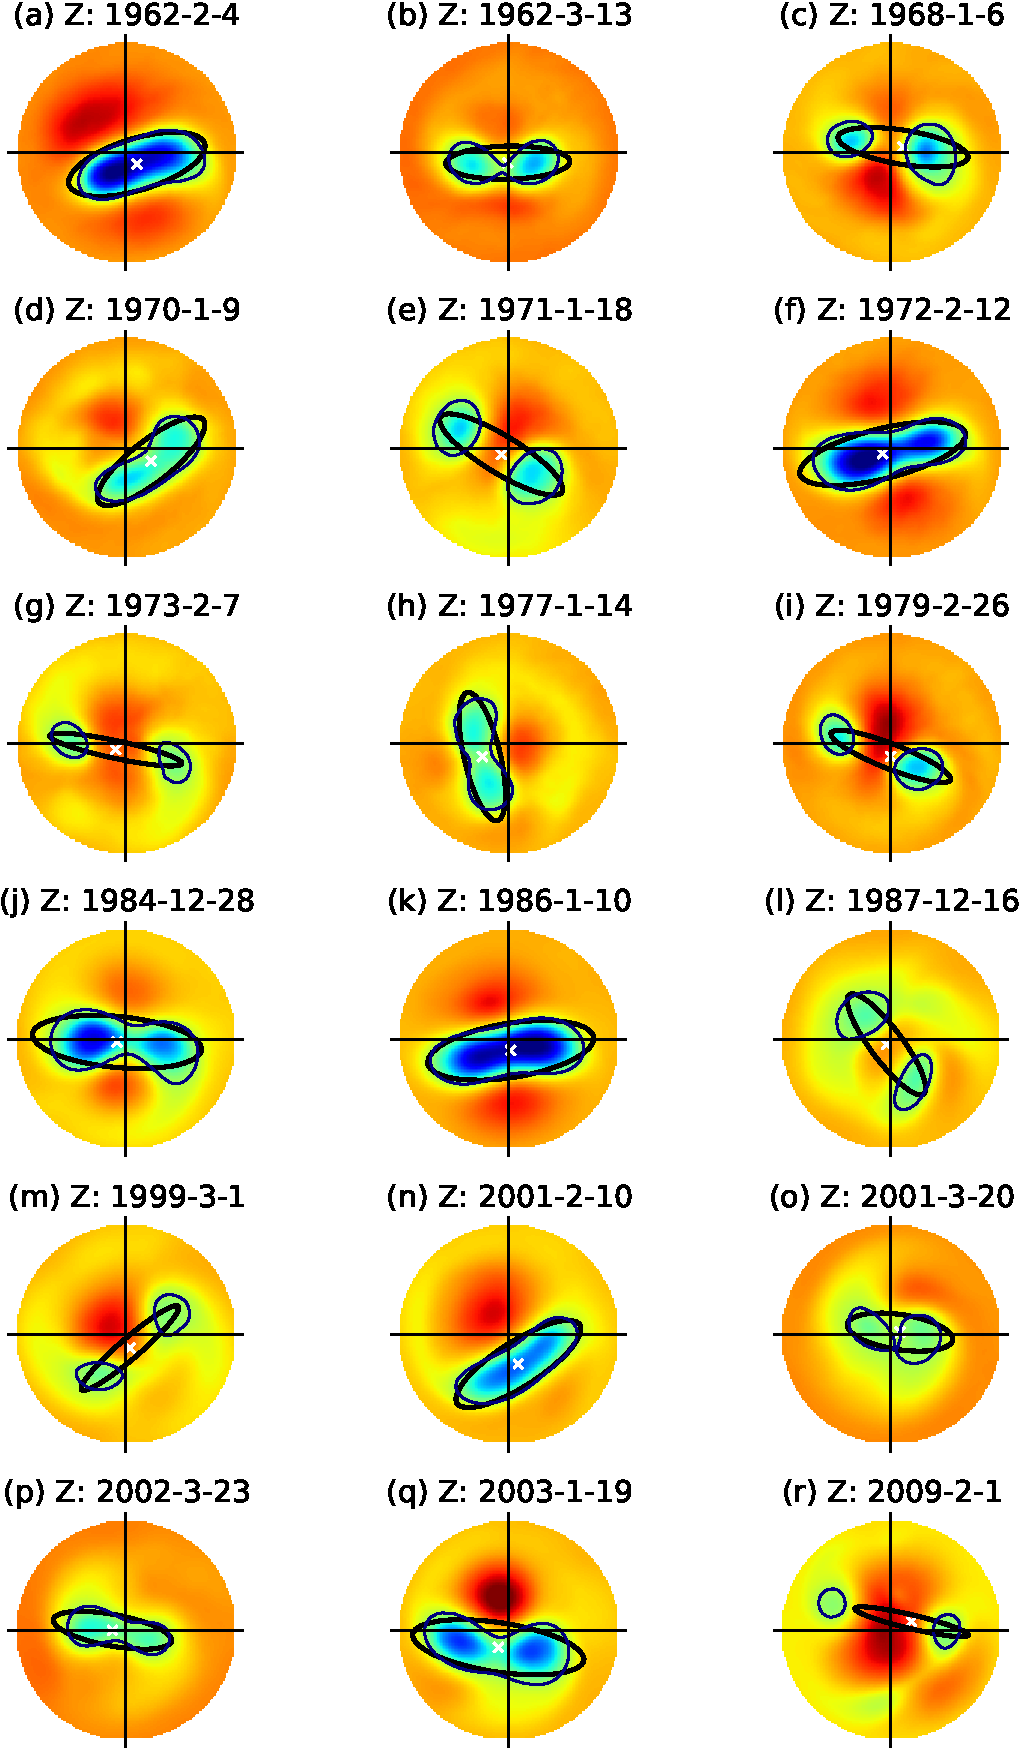
\includegraphics[width=0.8\textwidth]{figures/chapter-moments/GPH_all_events_splits.pdf}
 \caption[Geopotential height at the peak of split vortex events.]{10~hPa
   geopotential height at the peak of each of the 18 split vortex events
   identified in ERA. The peak is defined as the day with the largest aspect
   ratio during the two weeks following the onset date. The vortex edge is shown
   as a thin black contour, the equivalent ellipse the thick black contour and
   its centroid as a white cross. Data are transformed to cartesian coordinates
   with a polar stereographic projection.}
 \label{fig:gph_all_events_splits}
\end{figure}

\begin{figure}[htbp]
 \centering
 \noindent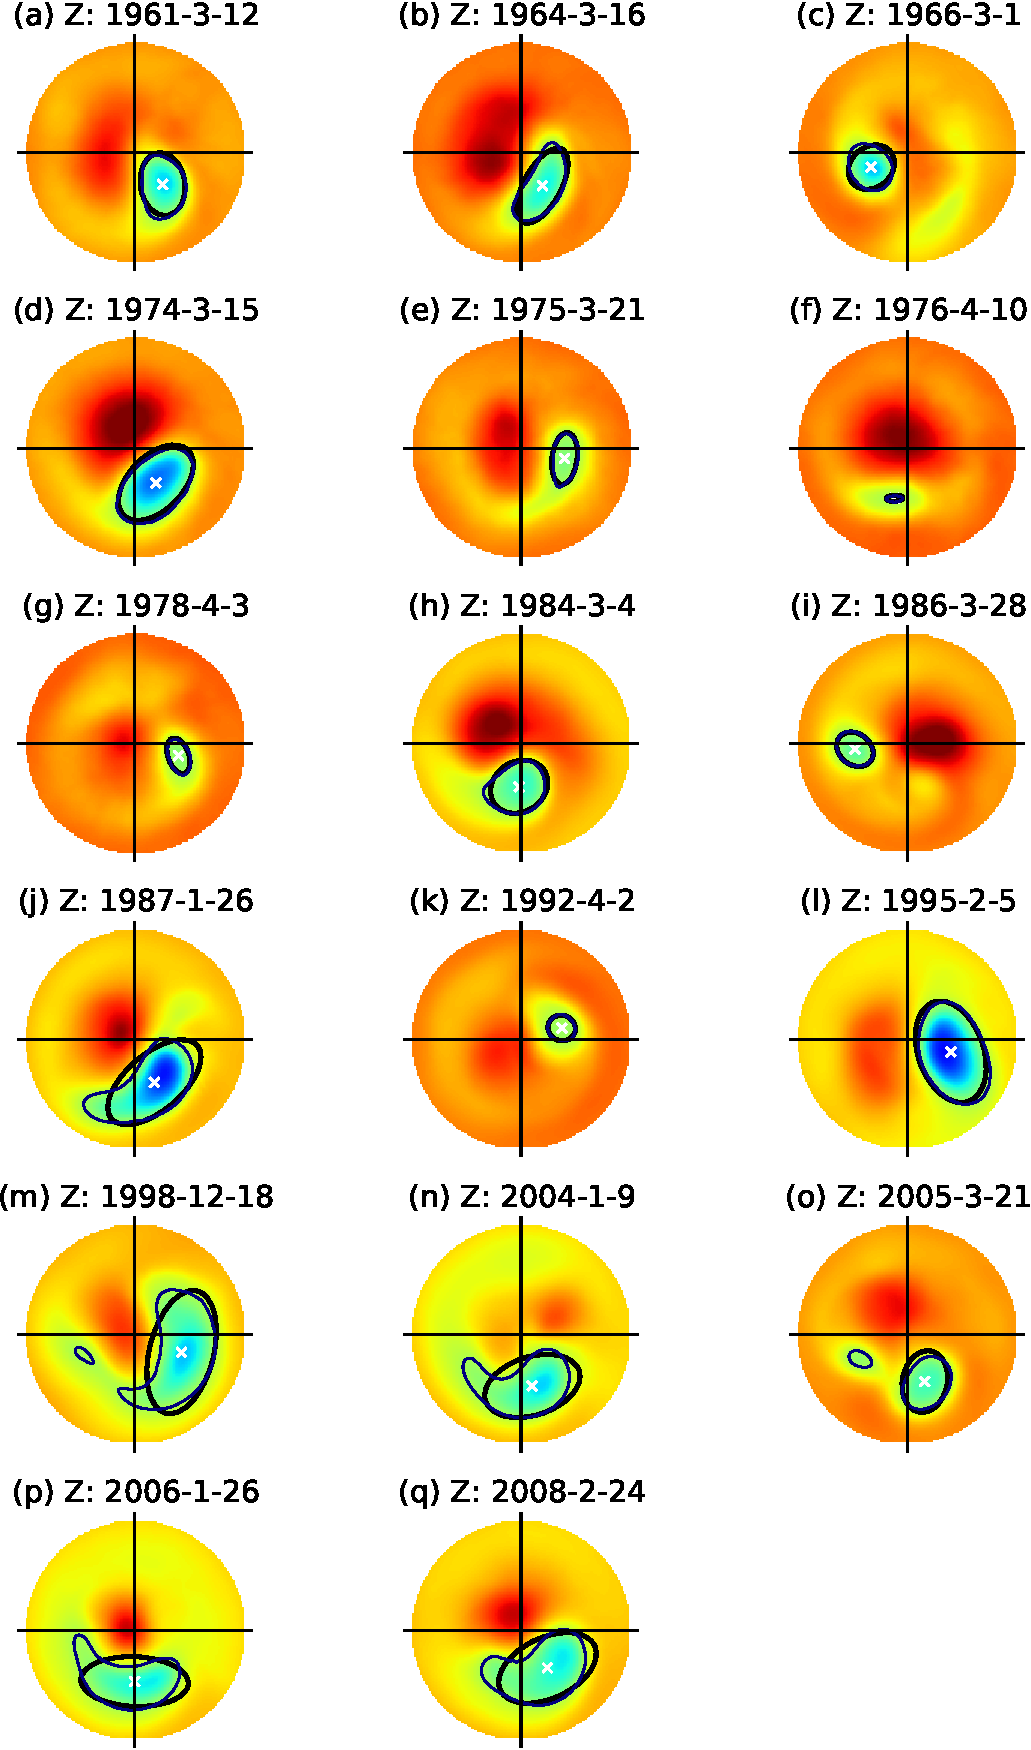
\includegraphics[width=0.8\textwidth]{figures/chapter-moments/GPH_all_events_displs.pdf}
 \caption[Geopotential height at the peak of displaced vortex events.]{As Figure
   \ref{fig:gph_all_events_splits} but for the 17 displaced vortex events
   identified in ERA.}
 \label{fig:gph_all_events_displs}
\end{figure}

Figures \ref{fig:gph_all_events_splits} and \ref{fig:gph_all_events_displs} show
geopotential height at the peak of each of the split and displaced vortex
events. The peak is defined as the day with the maximum aspect ratio or minimum
centroid latitude in the two weeks following the onset date of split and
displaced vortex events respectively. Almost all of the split vortex events show
two clearly separated vortices or a pinched vortex shape, which is approximately
symmetrical about the North Pole. Two exceptions are Figures
\ref{fig:gph_all_events_splits} (a) and (k), in which the vortex is highly
elliptical but not clearly split. Figure \ref{fig:gph_all_events_splits}(n)
shows an event with a highly elliptical vortex that is also somewhat displaced
from the pole, indicating that it has some displaced nature. The majority of
split vortex events are seen to occur along the $90^{\circ}$E-$90^{\circ}$W
axis, in line with the climatological wave-2 pattern \citep{Andrews1987}. Figure
\ref{fig:gph_all_events_splits}(h) shows an exception to this, with an
orientation orthogonal to the majority of events. 

The displacement events mostly show a smaller and weaker vortex, owing to the
fact that they are more common later in winter (see Figure
\ref{fig:z_m13_cp07_histogram}). Some events, particularly those occurring in
late March, are also likely to be events which would traditionally be defined as
final warmings. It can be seem that the majority of displacement events occur in
the direction of the 0-90$^{\circ}$E quadrant, again in line with the
climatological wave-1 pattern. However, there are some exceptions to this, for
instance Figures \ref{fig:gph_all_events_displs} (c) and (i), which  show a
westward-displaced vortex. 



\subsection{Comparison with CP07 and M13}

The split and displaced vortex events identified using the above method are now
compared with those of the CP07 and M13 methods. Table \ref{tab:events}
identifies those events which do not coincide with the events of CP07 and M13,
where `coincide' is taken to mean events within 10 days and of the same type. Of
the 35 events identified, 16 were found not to coincide with events of CP07 (10
displacement and 6 split). Six events were found not to coincide with those of
M13 (3 displacement and 3 split), although this comparison only covers the 28
events from 1958-2002, as it was not possible to reproduce the M13 method over
the longer period studied here because of the difficulties with hierarchical
clustering discussed in Section \ref{sec:event-definition}. Just two completely
new events were identified (i.e. not coinciding with either CP07 or M13); these
are the displaced vortex events with onset dates 1978-3-25 and 1995-2-2.

Table \ref{tab:events} also shows polar cap averaged 10~hPa temperature
anomalies ($\Delta \mathrm{T}_{10}$), averaged 5 days either side of the event
to give a measure of the event magnitude. The events of CP07 show a larger
average anomaly than events identified with the current method, although the two
are not statistically significantly different: CP07 average 8.6~K [6.1, 10.9]
split and 7.8~K [5.5, 9.9] for displaced vortex events, while the current method
averages 5.7~K [3.0, 8.3] for split and 6.8~K [5.5, 8.2] for displaced vortex
events (numbers in square brackets represent the 95\% uncertainty range,
calculated using a bootstrap test). It can be seen that while the vast majority
of events show positive values of $\Delta \mathrm{T}_{10}$ (i.e. warming), four
events show negative values. All of these events are also identified by M13, and
they attributed the negative values to the presence of a strong, cold vortex
prior to the event. Zonal-mean zonal wind at $60^{\circ}$N and 10~hPa
($\overline{U}_{10}$), averaged over the same period is also shown in Table
\ref{tab:events}. The majority of events show negative values, in line with the
traditional wind reversal criterion, although some show positive values. This
again may result from a strong vortex prior to these events, as well as the fact
that the current method may detect events with a distorted but strong vortex. 

% Mean values 
% -----------
% DT: Split: 5.7 pm 5.7 (3.0, 8.3)
%     Displ: 6.8 pm 2.9 (5.5, 8.2)
%     Split (CP07): 8.6 pm 4.6 (6.1, 10.9)
%     Displ (CP07): 7.8 pm 3.9 (5.5, 9.9)


The seasonal distribution of split and displaced vortex events identified by the
current method ($Z_{10}$), M13, and CP07, is shown in Figure
\ref{fig:z_m13_cp07_histogram}. In all three methods split vortex events are
more frequent in early-mid winter, with a peak in January. For displaced vortex
events, both the current method and M13 show a skew towards events occurring
later in winter. However, there is less similarity with the CP07 distribution of
displaced vortex events. CP07 indicates an approximately flat distribution
throughout winter, and many fewer displaced vortex events overall. It should be
noted that the seasonal distribution of split vortex events from the moment
based methods does not arise from the underlying climatology of aspect ratio,
which remains approximately constant throughout winter (e.g.,
\ref{fig:cmip5_moments_stats_seas}). The centroid latitude does however, show a
small equatorwards trend throughout winter, which may to some extent account for
the seasonal distribution of displaced vortex events \citep{Mitchell2011}.

\begin{figure}
  \centering
  \noindent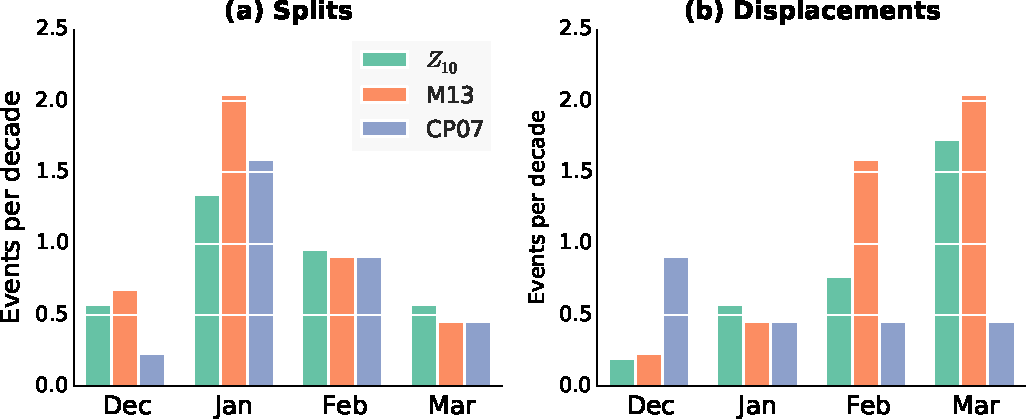
\includegraphics[width=\textwidth]{figures/chapter-moments/splits_displacements_histogram.pdf}
  \caption[Seasonal distribution of displaced and split vortex
  events.]{Histogram of the seasonal distribution of displaced and split vortex
    events, form the current ($Z_{10}$) method, M13 and CP07.}
  \label{fig:z_m13_cp07_histogram}
\end{figure}

Figure \ref{fig:pv_composites_m13_cp07} compares the average shape of the
stratospheric polar vortex following the split and displaced vortex events
identified by the three methods. Composites of PV in the mid-stratosphere
(850~K) are shown averaged 5 days following each event. For the split vortex
events, the current method ($Z_{10}$) method clearly shows two separated
vortices, one centred over Canada and the other over Siberia. For the M13 events
the split vortex composite shows the vortex stretched across the same
$90^{\circ}$W-$90^{\circ}$E line, although not as clearly split, while the
composite for the CP07 events looks very different. This has a weak vortex
centred over Canada, with the other over Northern Europe in a similar location
to the composite for displaced events. All three composites for displaced events
show a vortex centred over Northern Europe, but this extends most westward in
the CP07 composite, suggesting that there may be some contamination from
misdiagnosed split vortex events.

\begin{figure}
 \centering
 \noindent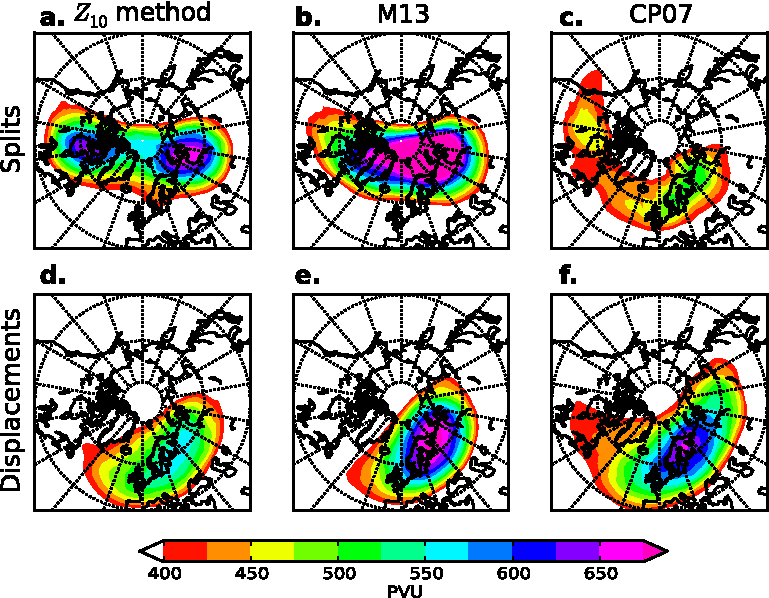
\includegraphics[width=\textwidth]{figures/chapter-moments/pv_composites_colbar_crop.pdf}
 \caption[PV composites for split and displaced vortex events.]{Composites of
   potential vorticity at the 850~K isentropic surface from the ERA reanalysis
   over 1958-2009. Composites are taken over the 5 days following the onset date
   of split vortex events (a,b,c) and displaced vortex events (d,e,f). The
   current ($Z_{10}$) method (a,b) is compared with that of M13 (b,e) and CP07
   (c,f).}
 \label{fig:pv_composites_m13_cp07}
\end{figure}

Overall, Figure \ref{fig:pv_composites_m13_cp07} demonstrates that the current
method succeeds (in a composite sense) in identifying displaced and split vortex
events events at least as well as the methods of M13 or CP07. When comparing the
three methods, CP07 is the clear outlier. This is most likely because the CP07
approach employs a zonal-mean threshold which cannot accurately capture some
extreme events (as discussed in M13).


\section{Influence on the troposphere}
\label{sec:moments_analysis}

\begin{figure}
 \centering
 \noindent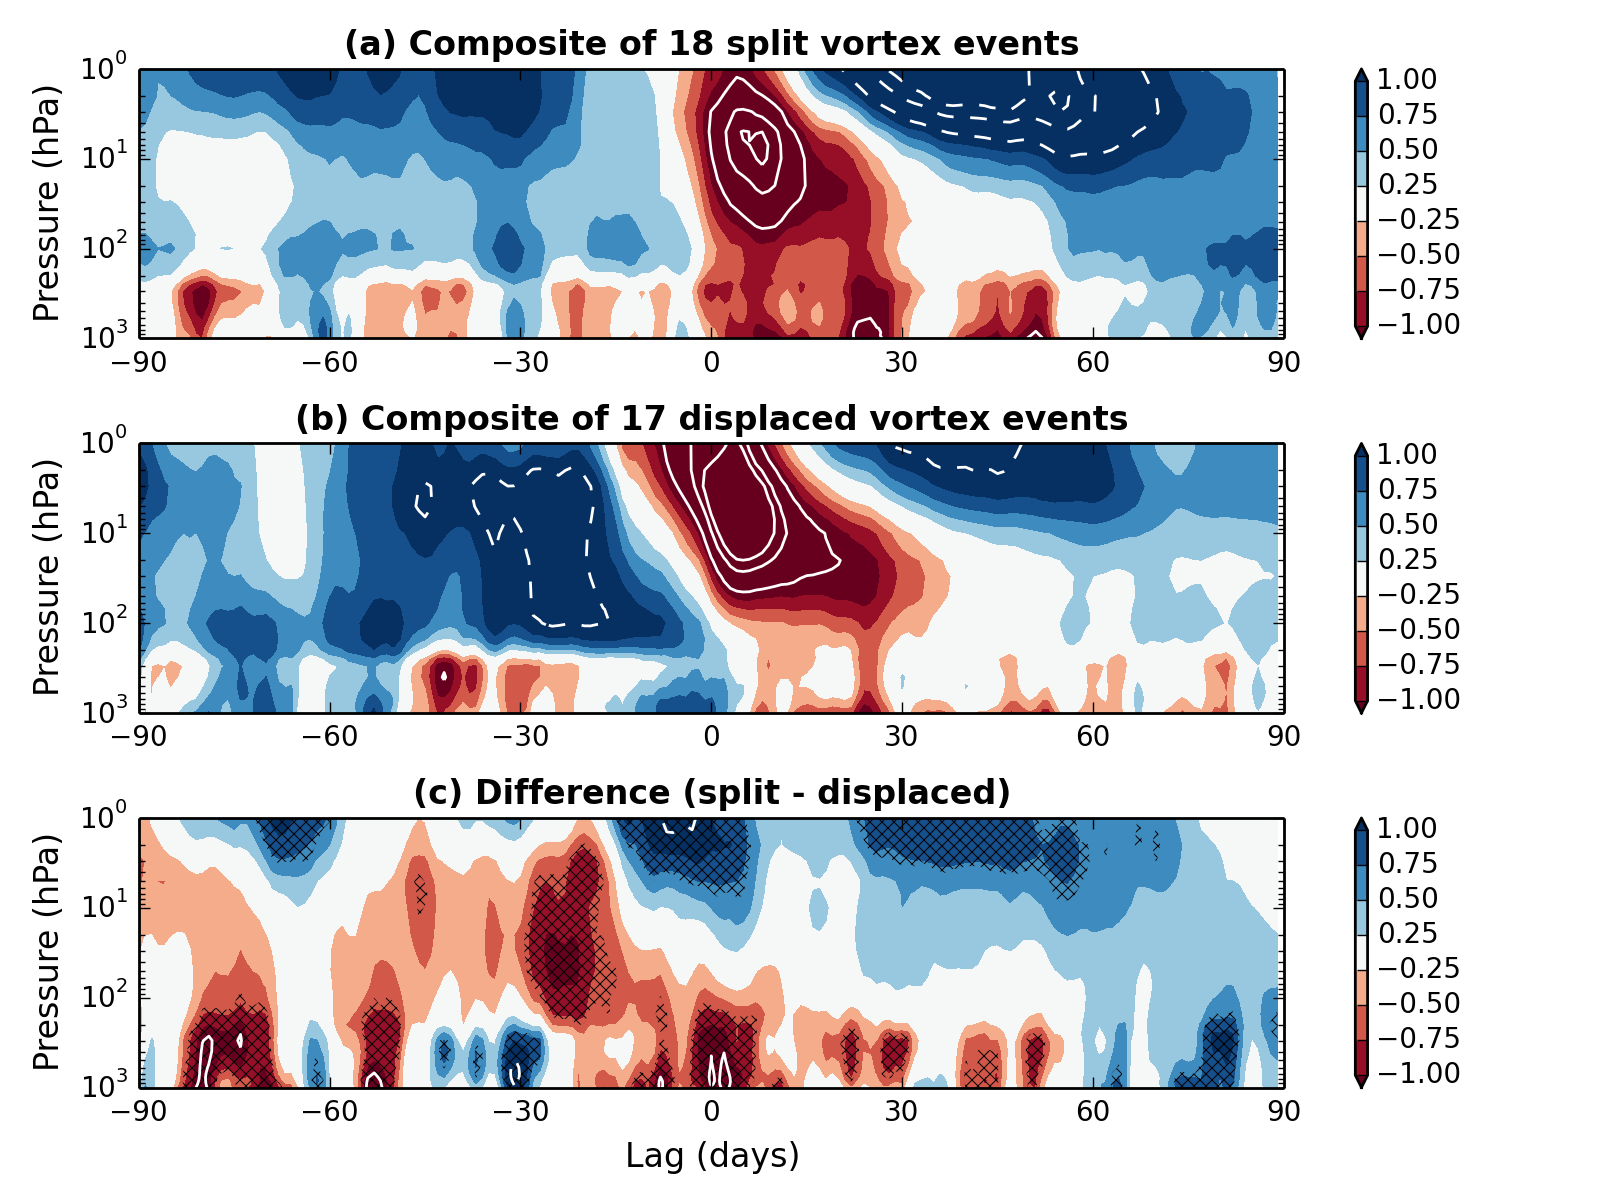
\includegraphics[width=\textwidth]{figures/chapter-moments/dripping_paint.png}
 \caption[NAM composites for split and displaced vortex events.]{Composites of
   the time-height evolution of the NAM during (a) 17 vortex displacement events
   and (b) 18 splitting events. (c) shows the difference in these composites,
   and hashed regions represent those that are 95\% significant according to a
   two-tailed bootstrap test. Lag 0 is at the onset of an event as measured at
   10 hPa. Contour intervals are 0.25 and the region between -0.25 and 0.25 is
   unshaded. Data is from the ECMWF Reanalyses 1958-2009.}
 \label{fig:dripping_paint}
\end{figure}

Having verified that this new method identifies split and displaced vortex
events as skillfully as previous methods, it is now possible to study their
influence on the troposphere. This is motivated by the result of M13 who, as
discussed in Section \ref{sec:observ-evid}, found tropospheric anomalies to be
larger following split vortex events that displaced vortex events. Figure
\ref{fig:dripping_paint}(a,b) shows time-height composites of the NAM over the
90 days following split and displaced vortex events. Here the method of
\citet{Baldwin2009} is used to define the NAM as the leading empirical
orthogonal function (EOF) of daily wintertime (November-April) zonal mean
geopotential height anomalies poleward of $20^{\circ}$N. The anomalies are
calculated by subtracting the seasonal cycle which has been smoothed with a
90-day low-pass filter. The daily NAM anomalies are then determined by
projecting daily geopotential anomalies onto the leading EOF patterns. Finally,
the NAM is normalised at each level so that the entire time series has unit
variance.

In agreement with M13, it can be seen that the tropospheric NAM is more negative
during the 60 days following split vortex events than displaced vortex
events. Also similar to M13 is the fact the vertical evolution for the two
events greatly differs, with split vortex events occurring almost instantaneously
throughout the depth of the atmosphere and displaced vortex taking almost two
weeks to propagate through the stratosphere. The near-barotropic nature of split
vortex events suggests that resonant excitation of the barotropic normal mode
\citep{Esler2005} is an important influence in this case. 
% Furthermore, the rapid onset of split vortex events is ... (Love 1893).

The difference in the NAM composites (split minus displaced) is shown in Figure
\ref{fig:dripping_paint}(c). Statistical significance in this difference is
calculated with the null hypothesis that there is no difference between the NAM
response to split and displaced vortex events, and assessed using a two tailed
bootstrap test with the following procedure:
\begin{enumerate}[i.]
\item The labels `split' and `displacement' are randomly re-assigned to the 35
  events.
\item NAM composites and the composite difference of these randomly assigned events
  are calculated. 
\item The above steps are repeated $10~000$ times, to form a distribution
  of random composite differences. If the true composite difference lies
  $<2.5\%$ or $>97.5\%$ within this distribution, then it can be said to be 95\%
  significant.
\end{enumerate}
Some significant differences are seem between the split and displaced vortex
composites. For instance, a more negative stratospheric NAM is seen to precede
displaced vortex events, while the dipole in the upper stratospheric and
tropospheric NAM near lag 0 represents the difference in baroclinicity of the
two types of event. Some regions of significant differences are seen in the
tropospheric NAM from 0-60 days, but there are also some regions that are not
significant. Care must be taken when interpreting the importance of small
significant regions these may arise by chance, even if no physical relationship
exists. 

\begin{figure}
 \centering
 \noindent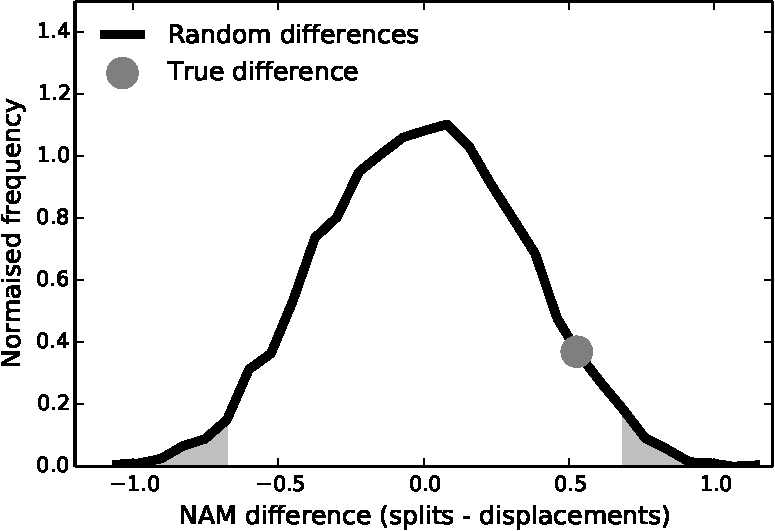
\includegraphics[width=0.7\textwidth]{figures/chapter-moments/nam_difference_sig.pdf}
 \caption[Significance of surface NAM difference following split and displaced
 vortex events.]{Distribution of 0-30 day mean NAM composite differences between
   split and displaced vortex events, formed by randomly shuffling the labels
   `split' and `displacement' between events. The 95\% significant region
   (according to a two-tailed test; i.e. $<2.5$\% and $>97.5$\%) is shaded and
   the true composite difference is at the 94th percentile.}
 \label{fig:nam_comp_diff}
\end{figure}

The difference in the tropospheric anomalies following split and displaced
vortex events is tested more robustly by examining surface anomalies averaged
over the 30 days following onset. This difference is again tested using the
bootstrap procedure outlined above. The distribution of randomly calculated
composite differences along with the true composite difference is shown in
Figure \ref{fig:nam_comp_diff}. It can be seen that the true NAM difference does
not lie in the 95\% significant region, so the null hypothesis that there is no
difference between anomalies following split and displaced vortex events cannot
be rejected. It should be noted that the statistical test here is different to
that carried out by M13. They tested whether the surface NAM following split and
displaced vortex events were different from randomly selected winter dates,
finding that anomalies following splits are, but those following displacements
are not. They did not, however, test the \emph{difference} between split and
displaced vortex events. 

\begin{figure}
 \centering
 \noindent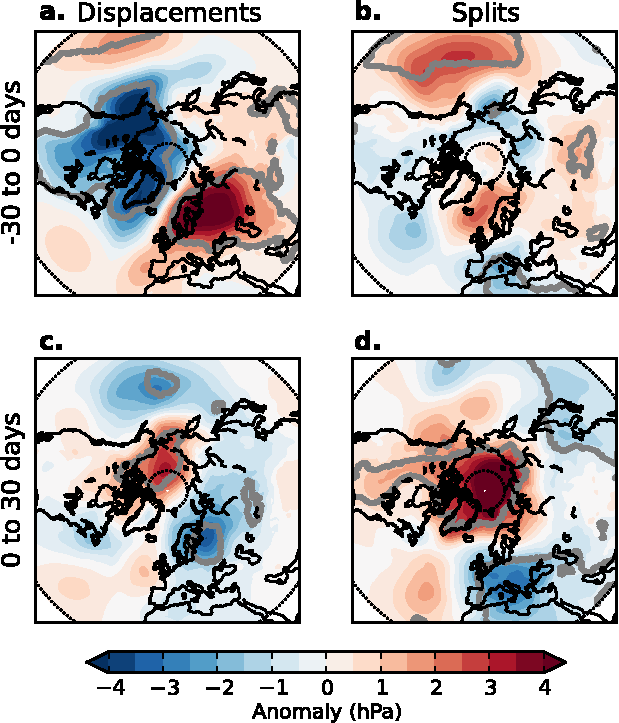
\includegraphics[width=0.7\textwidth]{figures/chapter-moments/mslp_composites_colbar_crop.pdf}
 \caption[Mean sea-level pressure composites for split and displaced vortex
 events.]{Composites of mean sea-level pressure anomalies in the 30 days before
   (a,b) and 30 days after (c,d) the onset dates of displaced (a,c) and split
   (b,d) vortex events from the $Z_{10}$ method. Data is from the ECMWF
   renalyses (1958-2009). Anomalies are calculated for each day and gridpoint
   from the climatology for that day of the year and gridpoint. Grey contours
   indicate regions of greater than 95\% statistical significance according to a
   bootstrap significance test.}
 \label{fig:mslp_composites}
\end{figure}

The NAM does not provide the full description of surface variability, and so in
Figure \ref{fig:mslp_composites} composites of MSLP 30 days before and 30 days
following the onset dates of displaced and split vortex events are
presented. Statistical significance is calculated against the null hypothesis
that anomalies before and after split and displaced vortex events are
indistinguishable from other winter dates. This is again estimated from a
two-tailed bootstrap test, in which $10~000$ composites of equal size are formed
from randomly selected winter dates, and the percentile of the true composite
calculated from this distribution. 

The strongest precursor is found for displaced vortex events, with a wave-1
pattern that is similar to the climatological stationary wave pattern
\citep[e.g.][]{Garfinkel2008}, suggesting increased wave-1 propagation into the
stratosphere. However, the strongest anomalies following events occur after
split vortex events, with a pattern resembling the negative phase of the NAM,
though with a southern centre of action shifted towards Europe. A further
difference between the split and displaced vortex composites is that their is a
more negative MSLP anomaly over Scandinavia and Siberia following displaced
vortex event. Overall, the main features of Figure \ref{fig:mslp_composites}
compare very well with the corresponding diagnostics from M13.

\begin{figure}
 \centering
 \noindent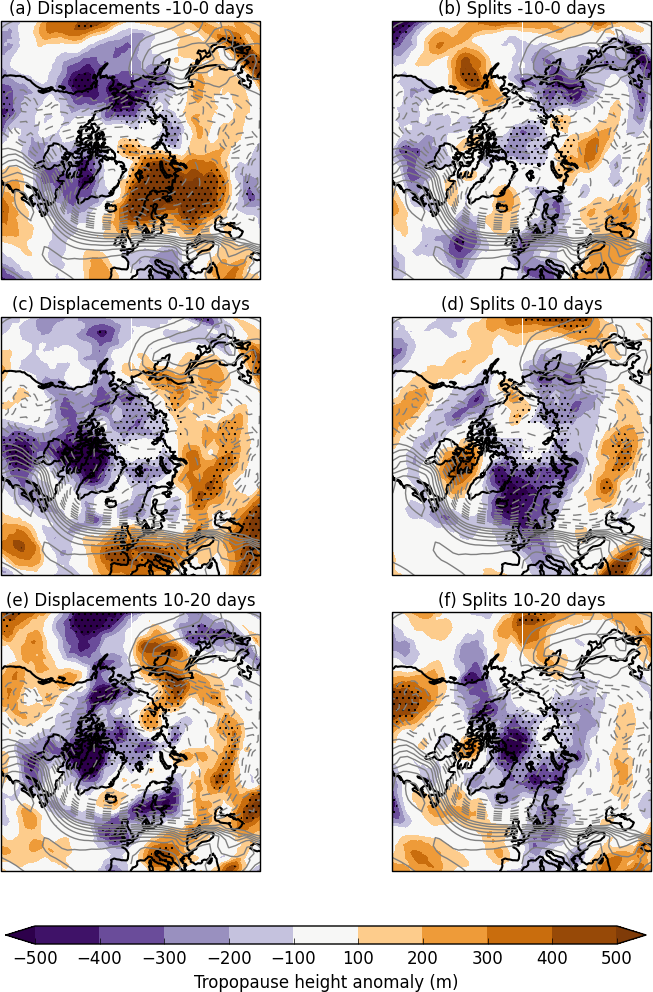
\includegraphics[width=0.8\textwidth]{figures/chapter-moments/tropopause_height_composites_nam_crop.png}
 \caption[Tropopause height composites for split and displaced vortex
 events.]{Composites of tropopause height anomalies averaged 10 days before
   (a,b), 10 days after (c,d) and 10-20 days after displaced and split vortex
   events. Anomalies are calculated for each day and gridpoint from the
   climatology for that day of the year and gridpoint. Stippling indicates
   regions of greater than 95\% statistical significance according to a
   Monte-Carlo significance test. Grey contours indicate the first EOF of NH
   mean sea-level pressure, which explains 33\% of the variance (dashes
   represent negative values).}
 \label{fig:tropopause_height}
\end{figure}

The mechanism of the stratosphere's influence on the troposphere proposed by
\citet{Ambaum2002} states that changes in the PV near the tropopause affect the
tropopause height and induce tropospheric anomalies below (more details are
given in Section \ref{sec:mechanisms}). In order to investigate this mechanism,
composites of tropopause height over the 10 days before, 10 days after, and
10-20 days after split and displaced vortex events are shown in Figure
\ref{fig:tropopause_height}. The measure of tropopause height used is that of
\citet{Wilcox2012a}, who construct a blended thermal and dynamical
tropopause. Significance is again calculated using a two-tailed bootstrap test. 

In line with the MSLP anomalies shown in Figure \ref{fig:mslp_composites},
tropopause height anomalies are seen to be larger prior to displaced vortex
events, with a wave-1-like structure. Following events, tropopause height
anomalies are seen to approximately mirror stratospheric PV anomalies (Figure
\ref{fig:pv_composites_m13_cp07}). That is, following displaced vortex events an
elevated tropopause is seen over Europe and Scandinavia, with a lowered
tropopause over Canada, and following split vortex events two regions of
elevated tropopause are present over Canada and Siberia with a depression
between. 

It is possible to quantitatively examine (although only approximately) whether
these tropopause anomalies are consistent with changes in stratospheric PV
above. Changes in tropopause pressure, $\Delta p_{\mathrm{trop}}$, are related
to changes in stratospheric PV, $\Delta q$, through
\begin{equation}
\Delta q \approx -q(1+\mathrm{Bu})\frac{\Delta
  p_{\mathrm{trop}}}{p_{\mathrm{trop}}} \, , 
\label{eqn:pv_trop}
\end{equation}
where $\mathrm{Bu}$ is the Burger number, which is approximately equal to one
for any PV anomaly \citep{Ambaum2002}. The change in tropopause height,
$\Delta h_{\mathrm{trop}}$ can be calculated using the hydrostatic relation
\begin{equation}
\Delta h_{\mathrm{trop}} = -\frac{\Delta p_{\mathrm{trop}}}{p_{\mathrm{trop}}}
\frac{R T_{\mathrm{trop}}}{g} \, , 
\end{equation} 
where $T_{\mathrm{trop}}$ is the tropopause temperature. Hence
\begin{equation}
\Delta h_{\mathrm{trop}} = \frac{\Delta q}{q}
\frac{RT_{\mathrm{trop}}}{g(1+\mathrm{Bu})} \, .
\end{equation}
Using a typical value of the PV change as $\sim 10\%$ (e.g., see Figure
\ref{fig:pv_composites_m13_cp07}), along with
$T_{\mathrm{trop}} = 210\mathrm{K}$, gives a change of tropopause height of
$\Delta h_{\mathrm{trop}} \approx 300\mathrm{m}$, which is indeed approximately
in line with the tropopause height anomalies seen in Figure
\ref{fig:tropopause_height}. This, along with the fact that the pattern in
tropopause height anomalies approximately mirrors that of stratospheric PV
anomalies, suggests that these tropopause height anomalies are induced by
changes in stratospheric PV above.

Also shown in Figure \ref{fig:tropopause_height} is the surface NAM pattern (the
leading EOF of DJFM daily MSLP). It can be seen that following split vortex
events more than displaced (especially days 0-10), the negative tropopause
height north of Iceland aligns more closely with the minimum in the NAM (this
region is also a node of the NAO). This may be significant if it is expected
that the fluctuation-dissipation theorem (FDT) holds in the tropospheric
response to stratospheric forcing. For systems in which the FDT holds, the
response of a system projected on a mode of variability should linearly scale
with the projection of the forcing on that mode \citep{Ring2008}. Under the
assumption that the tropopause height perturbation represents the ``forcing'',
this may project more strongly on the NAM/NAO following split vortex events,
consistent with a greater surface response to these events. Overall, however,
the pattern correlations between the split and displaced vortex tropopause
height anomalies and the NAM are not statistically significantly different
because the tropopause height field is very noisy. In order to give a more
detailed analysis a greater number of events would be needed.


 


\section{Conclusions}

Recent research has demonstrated the need to distinguish between split and
displaced stratospheric polar vortex events because of their different dynamics
and impacts on the troposphere. However, previous methods to identify these
events are impractical for application to climate model or seasonal prediction
simulations because they are highly sensitive to model climatology or rely on
non-standard variables. Motivated by this, we have developed a new method to
identify displaced and split vortex events which requires only geopotential
height at 10~hPa. The method is summarised as follows:
\begin{enumerate}[i.]
\item To identify the vortex region, a single contour of 10~hPa geopotential
  height is selected. This is the value of the DJFM mean zonal-mean at
  $60^{\circ}$N.
\item Using this contour the centroid latitude and aspect ratio moment
  diagnostics can be calculated.
\item Events are identified using a threshold criterion: Displaced events are
  occur if the centroid latitude remains equatorward $66^{\circ}$N for 7
  days or more. Split events occur if the aspect ratio remains above
  2.4 for 7 days or more. In order to ensure events are not counted twice, no
  two events may occur within 30 days.
\end{enumerate}
Vortex moment diagnostics derived from geopotential height are highly correlated
with those derived from PV, although fewer high aspect ratio values are
seen. The use of geopotential height here is motivated by the fact that it is
commonly output by climate models, whereas PV is not. However, in cases where PV
is available (such as in reanalyses) its use is preferable because of its
quasi-conservative properies and smaller-scale features. The above method can be
easily adapted to be used with PV-based vortex moments.

Analysis of the stratosphere following events identified by this method
demonstrates that it is able to accurately identify split and displaced vortex
events. Most of the events identified coincide with those of M13, and about
half with events identified by CP07. Composite analysis indicates that the
position of the stratospheric polar vortex following these events is at least as
extreme as that from the previous methods. 

Having identified these events, their impact on the troposphere is
investigated. Composites of the NAM indicate a more negative surface NAM over
the month following split vortex events than following displaced vortex
events. This supports the finding of M13, using a different event identification
method and extended data set. However, using a bootstrap test the composite
\emph{difference} of the surface NAM is not found to be statistically
significant.

Anomalies of tropopause height following split and displaced vortex events are
found to be co-located with stratospheric PV anomalies. They are also of a
magnitude consistent with being induced by changes in the stratospheric polar
vortex. Surface anomalies induced by changes in tropopause height may explain
therefore explain the different surface anomalies following split and displaced
vortex events. However, it is not possible to draw firm conclusions on this
because of the relatively small number of events and the noise of the MSLP and
tropopause height fields.

Overall, statistically significant results about the difference in the
tropospheric response to split and displaced vortex events will require a larger
number of events. This is achieved through the analysis of climate model
simulations in the next chapter.  

% ------------------- Copied from 2nd year report --------------%











%%% Local Variables:
%%% mode: latex
%%% TeX-master: "thesis"
%%% End:







